\chapter{Introduction}

\label{Chapter1_introduction} 

\begin{comment}
-------------------------------------------------
%								Chapter layout
1. Introduction
	a. Motivation
	b. Goals 
	c. Static Hand Gestures 
-------------------------------------------------
\end{comment}
%Computer science as a field is growing rapidly and expanding into many other disciplines including health care. This project is about very 
%short one paragraph or show explanation. maybe write abstract first. 

%------------------------------------------------
%	SECTION 1 Motivation
%------------------------------------------------
\section{Motivation}
Apraxia comes from the prefix “a” meaning “without” and the  Greek root word “praxis” which means “action”. Apraxia is a neurological condition that is sometimes caused by the effects of a stroke. It is a condition in which the patient is unable to exercise motor control over some of their muscles. The muscles themselves are not paralyzed or damaged, what causes these disorders are neurological conditions. In the department of Experimental Psychology researchers are studying patients with post-stroke loss of motor skills including possible cases of apraxia. The diagnosis of such a condition involves researchers presenting their patients with different movement based tests and evaluating the ease and effectiveness with which the patients are able to complete these screenings.  
	
%------------------------------------------------
%	SECTION 2 Goals
%------------------------------------------------
\section{Goals}
In the below paragraph, the general requirements for the working product of this project will be discussed. These requirements were elicited from the clinicians who will be the end users of this application when they use to collect hand gesture data from patients. The exact goals explained below were the result of several ongoing meetings during which different working versions of the software was shared with the clinicians for their input and suggestions.

The goals of this project are to create an application that can be used by clinicians at the John Radcliffe Hospital to diagnose patients for possible conditions of apraxia. This application should have a easy to use interface that allows the clinicians to collect data from patients easily. The data for each patient should be able to be stored in seperate folders by the ID of the patient. The application will also implement two algorithms that will score the attempted gesture data collected from patients. One of these algorithms will rely on comparing the relative angles between the two gestures being compared, and the other algorithm will break down a hand gesture into smaller components which themselves be scored and later a cumulative score can be given to the original gesture. The application should allow the clinicians to easily view the data that they collect within the application. It would be very useful if some of this data is editable from within the application to allow for mistakes to be corrected or comments to be written for certain gestures which were recorded. There should be an easy way to export and import the data in some common format such as CSV files so that the data can be analyzed in programs such as Excel. If possible, the application should design some method to account for the different variations in which the user's hand might be when they are completing gestures shown on the screen. 

%------------------------------------------------
%	SECTION 3 Static Hand Gestures 
%------------------------------------------------
\section{Static Hand Gestures}
The gestures this project will be concerned with are ten gestures for the left hand and ten gestures for the right hand. These specific gestures were provided by clinicians during the first meeting with them to discuss the scope of the project. Below are some pictures showing what the target gestures that the users will have to imitate will look like in application. The gestures shown are are the ten gestures for the left hand, along with a rotated version of the same gestures to provide a different perspective into the shape of the gesture. The right hand gestures will be mirror images of the ones shown below. 
%Gesture1Left
\begin{figure}[H]
    \centering
    \begin{minipage}{0.5\textwidth}
        \centering
        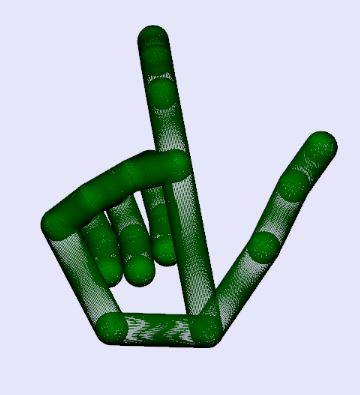
\includegraphics[scale=.75]{Figures/gesture1Left.JPG} 
        \caption[Gesture1Left]{Gesture1Left}
		\label{fig:Gesture1Left}
    \end{minipage}\hfill
    \begin{minipage}{0.5\textwidth}
        \centering
        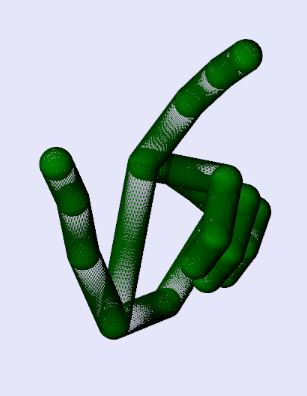
\includegraphics[scale=.7]{Figures/gesture1Left_rotated.JPG}
        \caption[Gesture1Left Rotated]{Gesture1Left rotated.}
        \label{fig:Gesture1Left_rotated}
    \end{minipage}
\end{figure}

%Gesture2Left
\begin{figure}[H]
    \centering
    \begin{minipage}{0.5\textwidth}
        \centering
        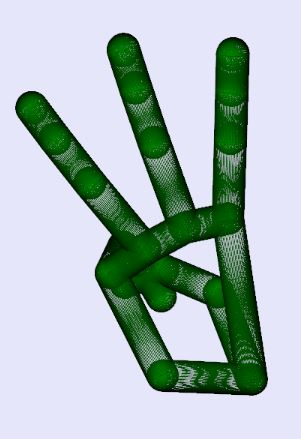
\includegraphics[scale=.75]{Figures/gesture2Left.JPG} 
        \caption[Gesture2Left]{Gesture2Left}
		\label{fig:Gesture2Left}
    \end{minipage}\hfill
    \begin{minipage}{0.5\textwidth}
        \centering
        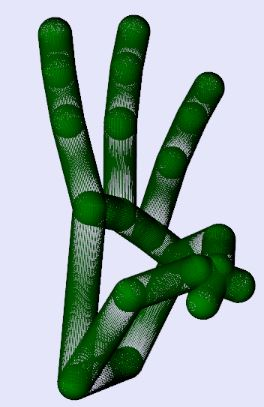
\includegraphics[scale=.75]{Figures/gesture2Left_rotated.JPG}
        \caption[Gesture2Left Rotated]{Gesture2Left rotated.}
        \label{fig:Gesture2Left_rotated}
    \end{minipage}
\end{figure}

%Gesture3Left
\begin{figure}[H]
    \centering
    \begin{minipage}{0.5\textwidth}
        \centering
        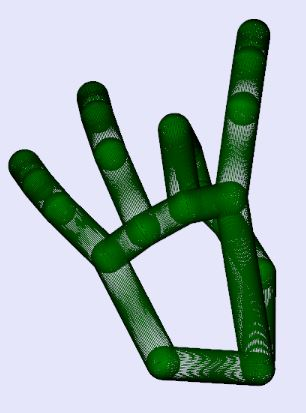
\includegraphics[scale=.75]{Figures/gesture3Left.JPG} 
        \caption[Gesture3Left]{Gesture3Left}
		\label{fig:Gesture3Left}
    \end{minipage}\hfill
    \begin{minipage}{0.5\textwidth}
        \centering
        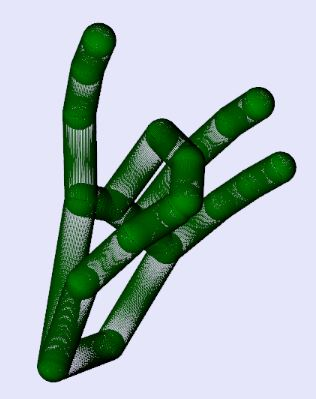
\includegraphics[scale=.75]{Figures/gesture3Left_rotated.JPG}
        \caption[Gesture3Left Rotated]{Gesture3Left rotated.}
        \label{fig:Gesture3Left_rotated}
    \end{minipage}
\end{figure}

%Gesture4Left
\begin{figure}[H]
    \centering
    \begin{minipage}{0.5\textwidth}
        \centering
        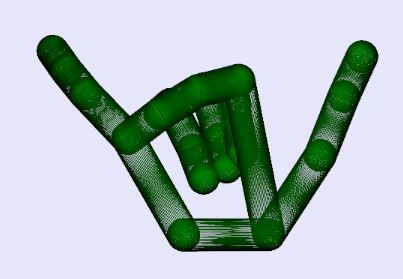
\includegraphics[scale=.75]{Figures/gesture4Left.JPG} 
        \caption[Gesture4Left]{Gesture4Left}
		\label{fig:Gesture4Left}
    \end{minipage}\hfill
    \begin{minipage}{0.5\textwidth}
        \centering
        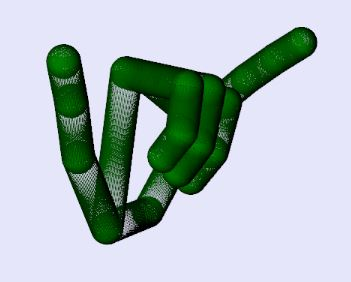
\includegraphics[scale=.75]{Figures/gesture4Left_rotated.JPG}
        \caption[Gesture4Left Rotated]{Gesture4Left rotated.}
        \label{fig:Gesture4Left_rotated}
    \end{minipage}
\end{figure}

%Gesture5Left
\begin{figure}[H]
    \centering
    \begin{minipage}{0.5\textwidth}
        \centering
        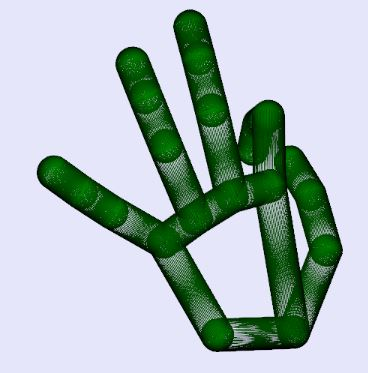
\includegraphics[scale=.75]{Figures/gesture5Left.JPG} 
        \caption[Gesture5Left]{Gesture5Left}
		\label{fig:Gesture5Left}
    \end{minipage}\hfill
    \begin{minipage}{0.5\textwidth}
        \centering
        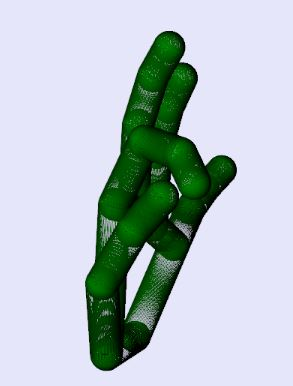
\includegraphics[scale=.75]{Figures/gesture5Left_rotated.JPG}
        \caption[Gesture5Left Rotated]{Gesture5Left rotated.}
        \label{fig:Gesture5Left_rotated}
    \end{minipage}
\end{figure}

%Gesture6Left
\begin{figure}[H]
    \centering
    \begin{minipage}{0.5\textwidth}
        \centering
        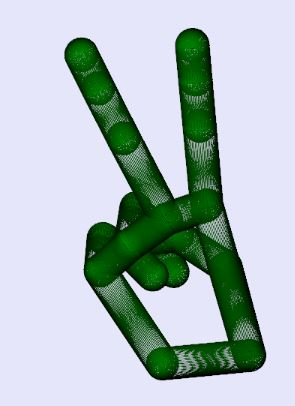
\includegraphics[scale=.75]{Figures/gesture6Left.JPG} 
        \caption[Gesture6Left]{Gesture6Left}
		\label{fig:Gesture6Left}
    \end{minipage}\hfill
    \begin{minipage}{0.5\textwidth}
        \centering
        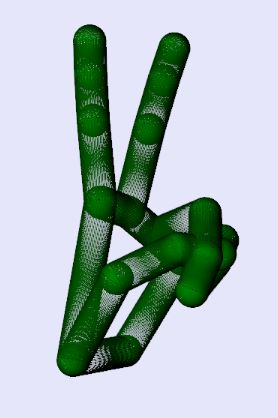
\includegraphics[scale=.7]{Figures/gesture6Left_rotated.JPG}
        \caption[Gesture6Left Rotated]{Gesture6Left rotated.}
        \label{fig:Gesture6Left_rotated}
    \end{minipage}
\end{figure}

%Gesture7Left
\begin{figure}[H]
    \centering
    \begin{minipage}{0.5\textwidth}
        \centering
        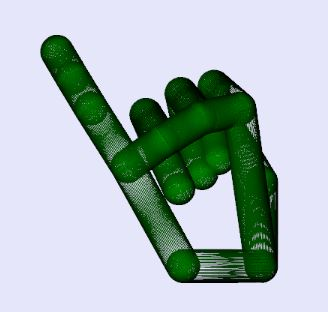
\includegraphics[scale=.75]{Figures/gesture7Left.JPG} 
        \caption[Gesture7Left]{Gesture7Left}
		\label{fig:Gesture7Left}
    \end{minipage}\hfill
    \begin{minipage}{0.5\textwidth}
        \centering
        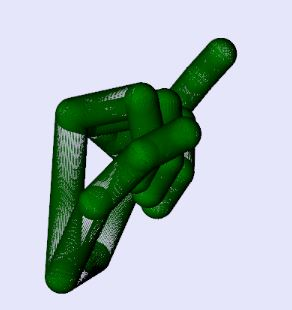
\includegraphics[scale=.75]{Figures/gesture7Left_rotated.JPG}
        \caption[Gesture7Left Rotated]{Gesture7Left rotated.}
        \label{fig:Gesture7Left_rotated}
    \end{minipage}
\end{figure}

%Gesture8Left
\begin{figure}[H]
    \centering
    \begin{minipage}{0.5\textwidth}
        \centering
        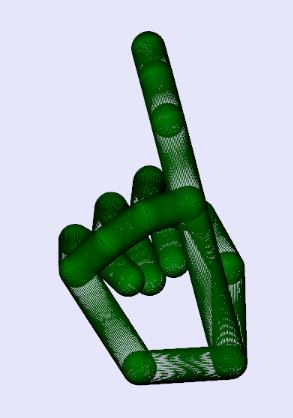
\includegraphics[scale=.75]{Figures/gesture8Left.JPG} 
        \caption[Gesture8Left]{Gesture8Left}
		\label{fig:Gesture8Left}
    \end{minipage}\hfill
    \begin{minipage}{0.5\textwidth}
        \centering
        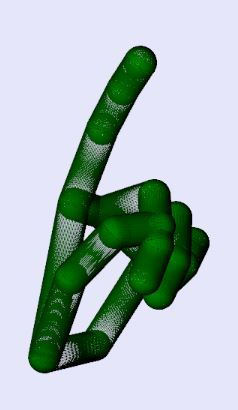
\includegraphics[scale=.75]{Figures/gesture8Left_rotated.JPG}
        \caption[Gesture8Left Rotated]{Gesture8Left rotated.}
        \label{fig:Gesture8Left_rotated}
    \end{minipage}
\end{figure}

%Gesture9Left
\begin{figure}[H]
    \centering
    \begin{minipage}{0.5\textwidth}
        \centering
        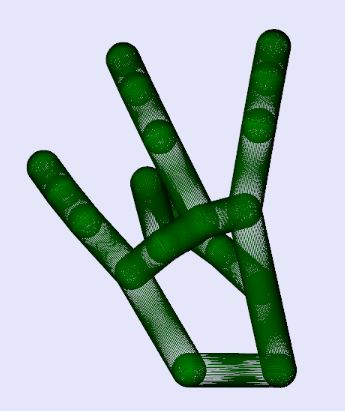
\includegraphics[scale=.75]{Figures/gesture9Left.JPG} 
        \caption[Gesture9Left]{Gesture9Left}
		\label{fig:Gesture9Left}
    \end{minipage}\hfill
    \begin{minipage}{0.5\textwidth}
        \centering
        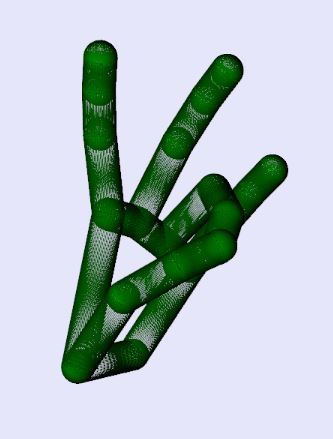
\includegraphics[scale=.75]{Figures/gesture9Left_rotated.JPG}
        \caption[Gesture9Left Rotated]{Gesture9Left rotated.}
        \label{fig:Gesture9Left_rotated}
    \end{minipage}
\end{figure}

%Gesture10Left
\begin{figure}[H]
    \centering
    \begin{minipage}{0.5\textwidth}
        \centering
        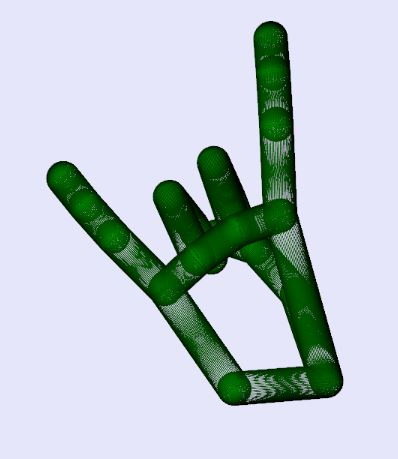
\includegraphics[scale=.75]{Figures/gesture10Left.JPG} 
        \caption[Gesture10Left]{Gesture10Left}
		\label{fig:Gesture10Left}
    \end{minipage}\hfill
    \begin{minipage}{0.5\textwidth}
        \centering
        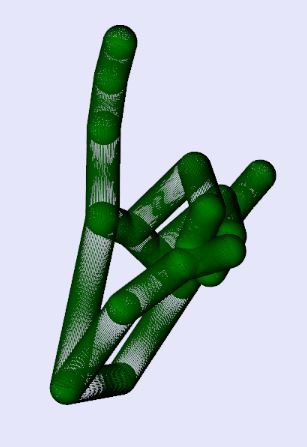
\includegraphics[scale=.75]{Figures/gesture10Left_rotated.JPG}
        \caption[Gesture10Left Rotated]{Gesture10Left rotated.}
        \label{fig:Gesture10Left_rotated}
    \end{minipage}
\end{figure}
